\documentclass[UTF8]{ctexart}
\usepackage{amsmath}
\usepackage{xfrac}
\usepackage{graphicx}
\usepackage{float}
\usepackage{listings}
\lstset{language=Matlab}

\title{动态规划求解0-1背包问题}
\author{U201715825 \quad 管实-江诗毅}
\date{\today}

\begin{document}
\maketitle
\tableofcontents

\newpage
\begin{abstract}
	首先根据0-1背包问题的描述给出了该问题的两种动态规划方程式(修正了老师给出的表达式),然后使用matlab实现了上述两种算法,分别验证了其时间复杂度,并且对比了两种方案的差异之处。
	
	然后,根据一种启发式贪心算法,描述了解决问题的思路,使用matlab实现,并分析了其优劣。
	
	最后,总结了实验收获。
\end{abstract}
\textbf{关键词:} 动态规划
\newpage
\section{动态规划一}
\subsection{方程式}
其他参数不变,原方程忽略了不加入物品的情况,故将动态规划方程式变为:
\[ g(x) = \max_{i:w_i \leq x} \{ v_i + g(x-w_i) , g(x-1) \} \]

\subsection{给出用法及验证时间复杂度}
\textbf{确定参数及用法}
\begin{lstlisting}
%knapsack 使用动态规划求解0-1背包问题
%
%输入:
%   v(vector) : 每个物品的价值
%   w(vector) : 每个物品的重量
%   x(vector) : 背包的容量
%
%输出:
%   plan(vector) : 逻辑1或者逻辑0向量,表示是否选择该物品
%   opt(number) : 最优的物品价值
\end{lstlisting}

实现思路会在下一小节谈到,这里先验证使用该动态规划方程得出的算法的时间复杂度为 \(O(nx)\),其中n为物品的个数,x为背包的容量大小。

绘制时间随规模--nx衡量的散点图,并用一次函数拟合,结果如下图(图1,图2).

由图可知,该算法的时间复杂度能较好的使用\( O(nx) \)来描述,下一小节会解释原因,以及其内存的耗费(空间复杂度).


\begin{figure}[H] %[htbp]
	\centering
	\begin{minipage}[t]{1\textwidth}
		\centering
		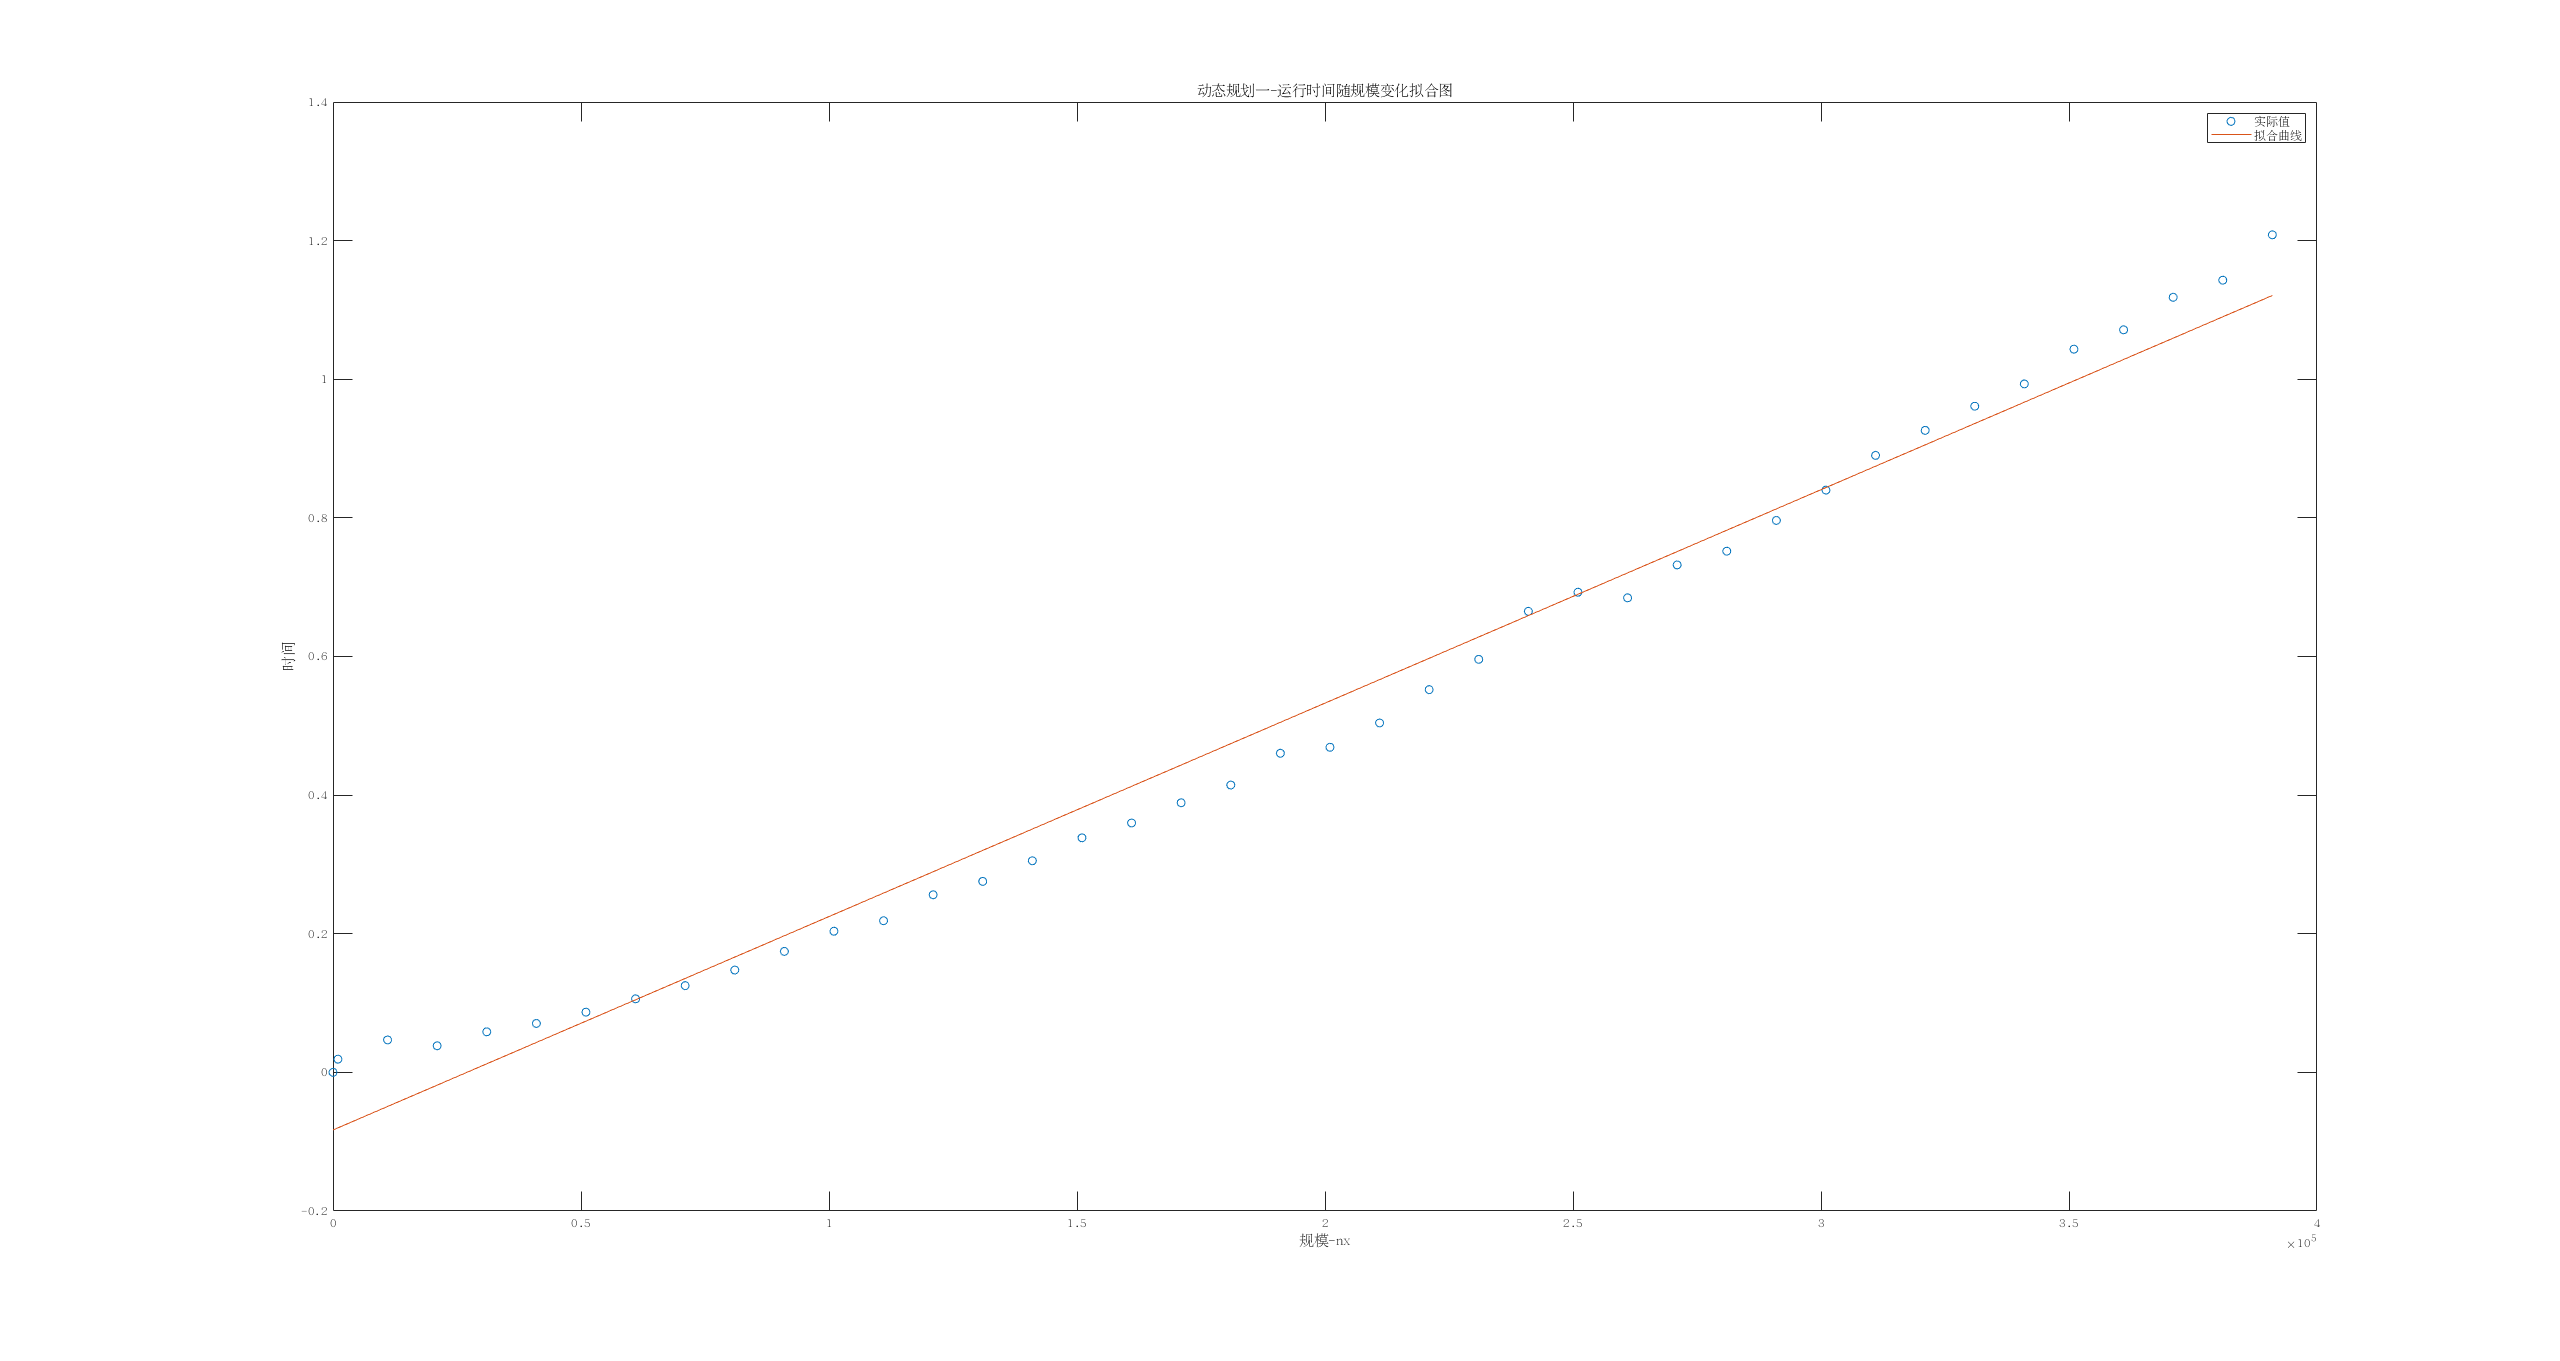
\includegraphics[width=10cm]{1.png}
		\caption{稀疏点拟合}
	\end{minipage}
	\begin{minipage}[t]{1\textwidth}
		\centering
		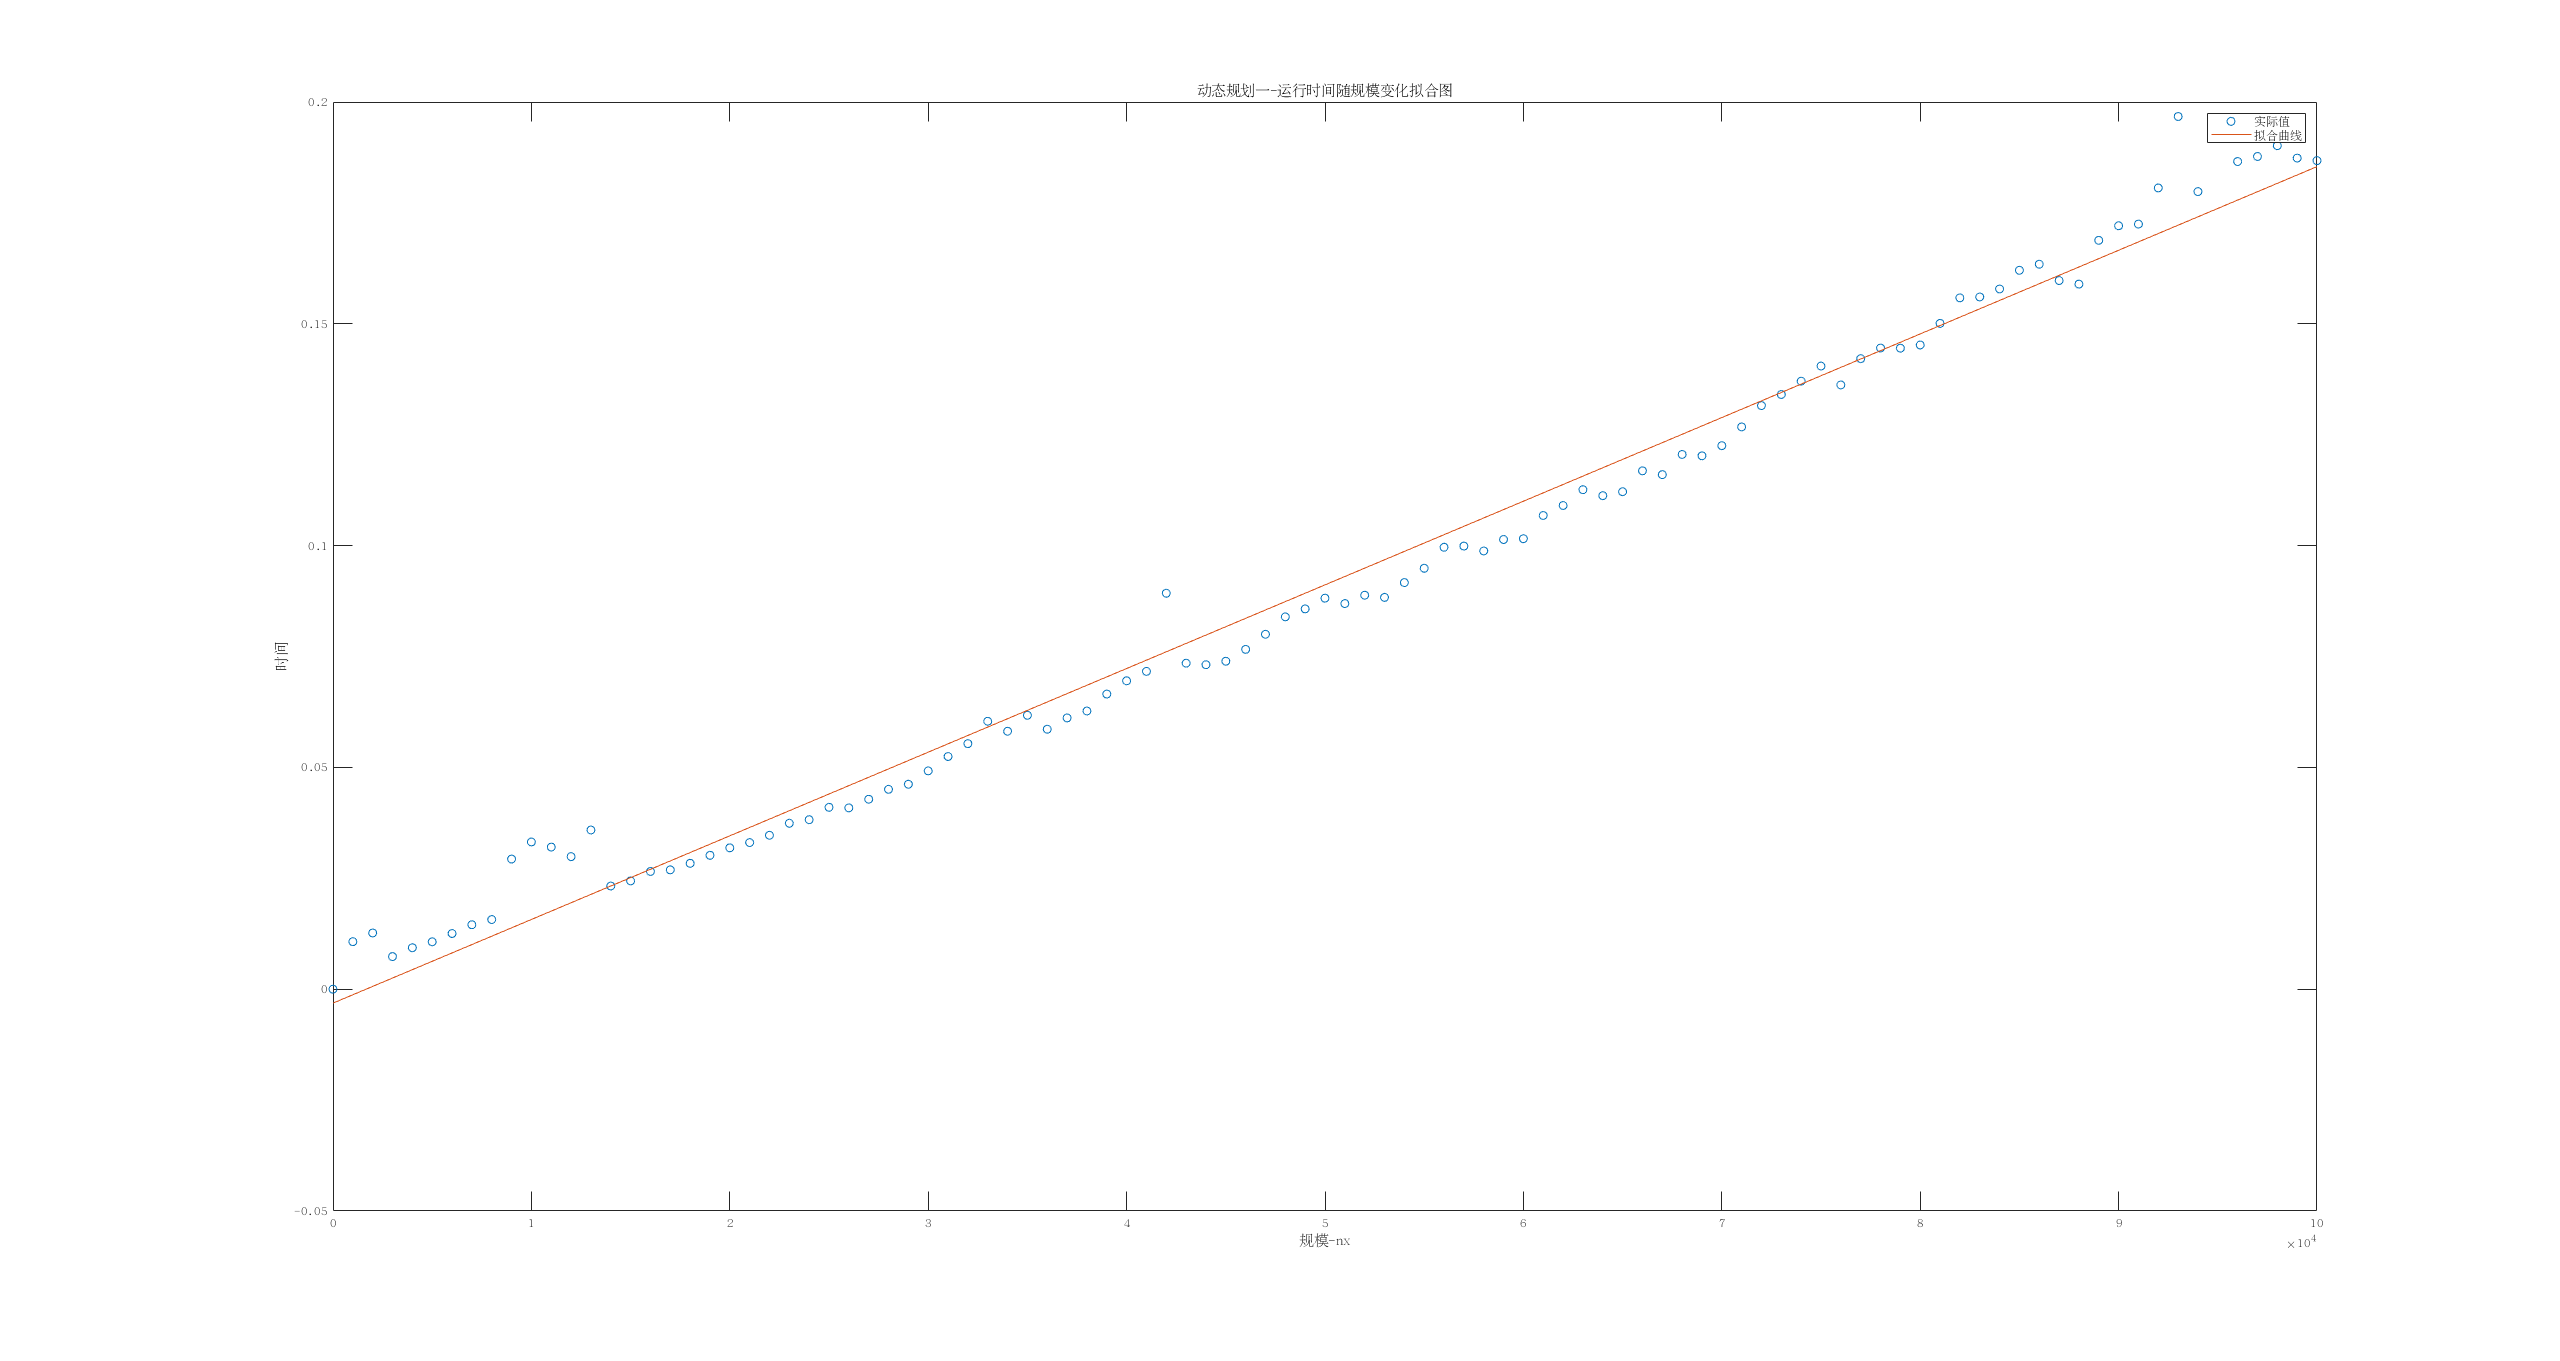
\includegraphics[width=10cm]{2.png}
		\caption{密集点拟合}
	\end{minipage}
\end{figure}


\subsection{实现思路}
实现思路:将求g(x)的最大值转换成求一个个小问题,背包容量从0到x逐步求出当前容量下的最优值(并且将子问题的最优选品方案存储起来),这样逐一迭代就能给出g(x)的最优值及其选品方案。

步骤:
\begin{itemize}
	\item 预分配内存:一个\( 1×(x+1) \)一维数组resultArr用来存储子问题的最优值,一个\( (x+1)×n \)二维数组s用来存储每个子问题的选品方案。
	\item 从0迭代到x,逐一选择比当前背包容量小的物品放入(或者不选任何物品)。将该物品的价值 加上当前容量减去该物品重量 这个子问题的最优值。
	\item 去掉重选,如果选择了一物品,并且该物品在子问题进行了选择,那么就不考虑该种方案。
	\item 从上述方案中选择价值最大的方案,这就是当前背包容量下的最优选品方案。
    \item 这样,最优值resultArr(x),最优的决策方案就是s(x,:)。
\end{itemize}
\textbf{伪代码}
\begin{lstlisting}
预分配内存resultArr,s
for i=1 to x
    resultArr(i+1) = resultArr(i);  % 这就是不选物品的最优值。
    s(i+1,:) = s(i,:);  % 更改最优方案。
	
    % 找到所有重量比x小并且前面没有用到的物品的索引
    for j = 重量比i小的物品索引
        if 物品在前面用过
        continue;
    end

    % 比较选出价值最大的方案。
    if 当前的方案比之前的优
        % 更新方案
        resultArr(i+1) = v(j) + resultArr(i-w(j)+1);
        s(i+1,:) = s(i-w(j)+1,:); 
        s(i+1,j) = 1;
\end{lstlisting}
\textbf{时间空间复杂度分析}

用伪代码的迭代语句中能够看出,首先是对1到x的背包容量进行了迭代,然后在每一种背包容量下对每一个物品进行了查找。共有n个物品,故算法的时间复杂度为\(O(n)\)。

内存开销,用到了一个\( 1×(x+1) \)一维数组,一个\( (x+1)×n \)二维数组,故空间复杂度为\( (x+1)(n+1)  \)

\subsection{测试用例}
为了较好的验证算法的正确性,我使用了DP1与DP3(任务3中的动态规划)做对比,(见test.m),发现它们给出的解答在少数情况下是不相同的。

例如,当

重量向量为[24    41    22    32    33    43    21    18     5     3    16    28    24     4    41     1    28    41    22    34]

价值向量为[4    29    19    27    26     7    32    17    14     1    26    15    11    37    32    17    20     6    27    27]

DP1得到的解为305,DP3得到的最优解为306,也就是说其中一个DP存在问题。下一节阐述DP1的问题所在。


\subsection{由测试用例发现的问题}
前面说到,DP1得到的最优解有问题,于是重新check代码,发现这个DP方程对0-1背包问题来说有一个问题,那就是在后面选择物品的时候,可能该物品已经在子问题中选择过了,而我采取的办法是直接将这种方案从整个可行解集中去掉。这样就带来错误。正确的做法是将这种重复选择的物品的重量从容量中减去,并且在子问题中也不考虑这种物品。这样就不符合DP方程的定义了。

于是更改0-1背包问题为0-n背包问题,也就是说每个物品可以选择多个,而不是一个,同样最优方案用一维数组表示,第i个位置的值表示选择了该物品几次。

\textbf{更改后的代码}
\begin{lstlisting}
function [plan,opt] = correctKnapsack(v,w,x)
%correctKnapsack    纠正1中的0-1背包问题解法,改为物品个数无限。
%
%输入:
%   v(vector) : 每个物品的价值
%   w(vector) : 每个物品的重量
%   x(vector) : 背包的容量
%
%输出:
%   plan(vector) : 表示第i个物品选了几个
%   opt(number) : 最优的物品价值
    leng = length(v);
    resultArr = zeros(1,x+1);  % g(x)的结果
    s = zeros(x+1,leng);  % 路线
    
    for i = 1:x
        % 赋一个初值 
        resultArr(i+1) = resultArr(i);
        s(i+1,:) = s(i,:);
        for j = find(w<=i)  % 找到所有重量比x小的索引
            if v(j) + resultArr(i-w(j)+1) > resultArr(i+1)
                resultArr(i+1) = v(j) + resultArr(i-w(j)+1);
                s(i+1,:) = s(i-w(j)+1,:); 
                s(i+1,j) = s(i+1,j) + 1;
            end
        end
    end    
    plan = s(i+1,:);
    opt = resultArr(x+1);
end
\end{lstlisting}

同样针对上面的例子:

重量向量为[24    41    22    32    33    43    21    18     5     3    16    28    24     4    41     1    28    41    22    34]

价值向量为[4    29    19    27    26     7    32    17    14     1    26    15    11    37    32    17    20     6    27    27]

对于容量25,得出的结果为:[0     0     0     0     0     0     0     0     0     0     0     0     0     0     0    25     0     0     0     0],很容易验证这是正确的。

\section{动态规划二}
\subsection{方程式}
针对另一种动态规划解法,相当于从两个维度进行分割成子问题。一个维度是物品的种类,从只有一个物品到包含所有物品。另一个维度是从背包的容量,从0容量到x容量。

\[G(m,x) = \max\{ G(m-1,x), G(m-1,x-w_m) + v_m \} \]
该动态规划方程的含义简单的理解,就是对于新增加的第m个物品,我可以选或者不选。

\subsection{给出用法及验证时间复杂度}
用法以及验证过程同上,不再赘述,只给出图示。

由图3,图4大致能看出这种动态规划算法时间复杂度也符合\( O(nx) \),并且耗时少于第一种动态规划。原因后再后面进行论述。
\begin{figure}[H] %[htbp]
    \centering
    \begin{minipage}[t]{1\textwidth}
        \centering
        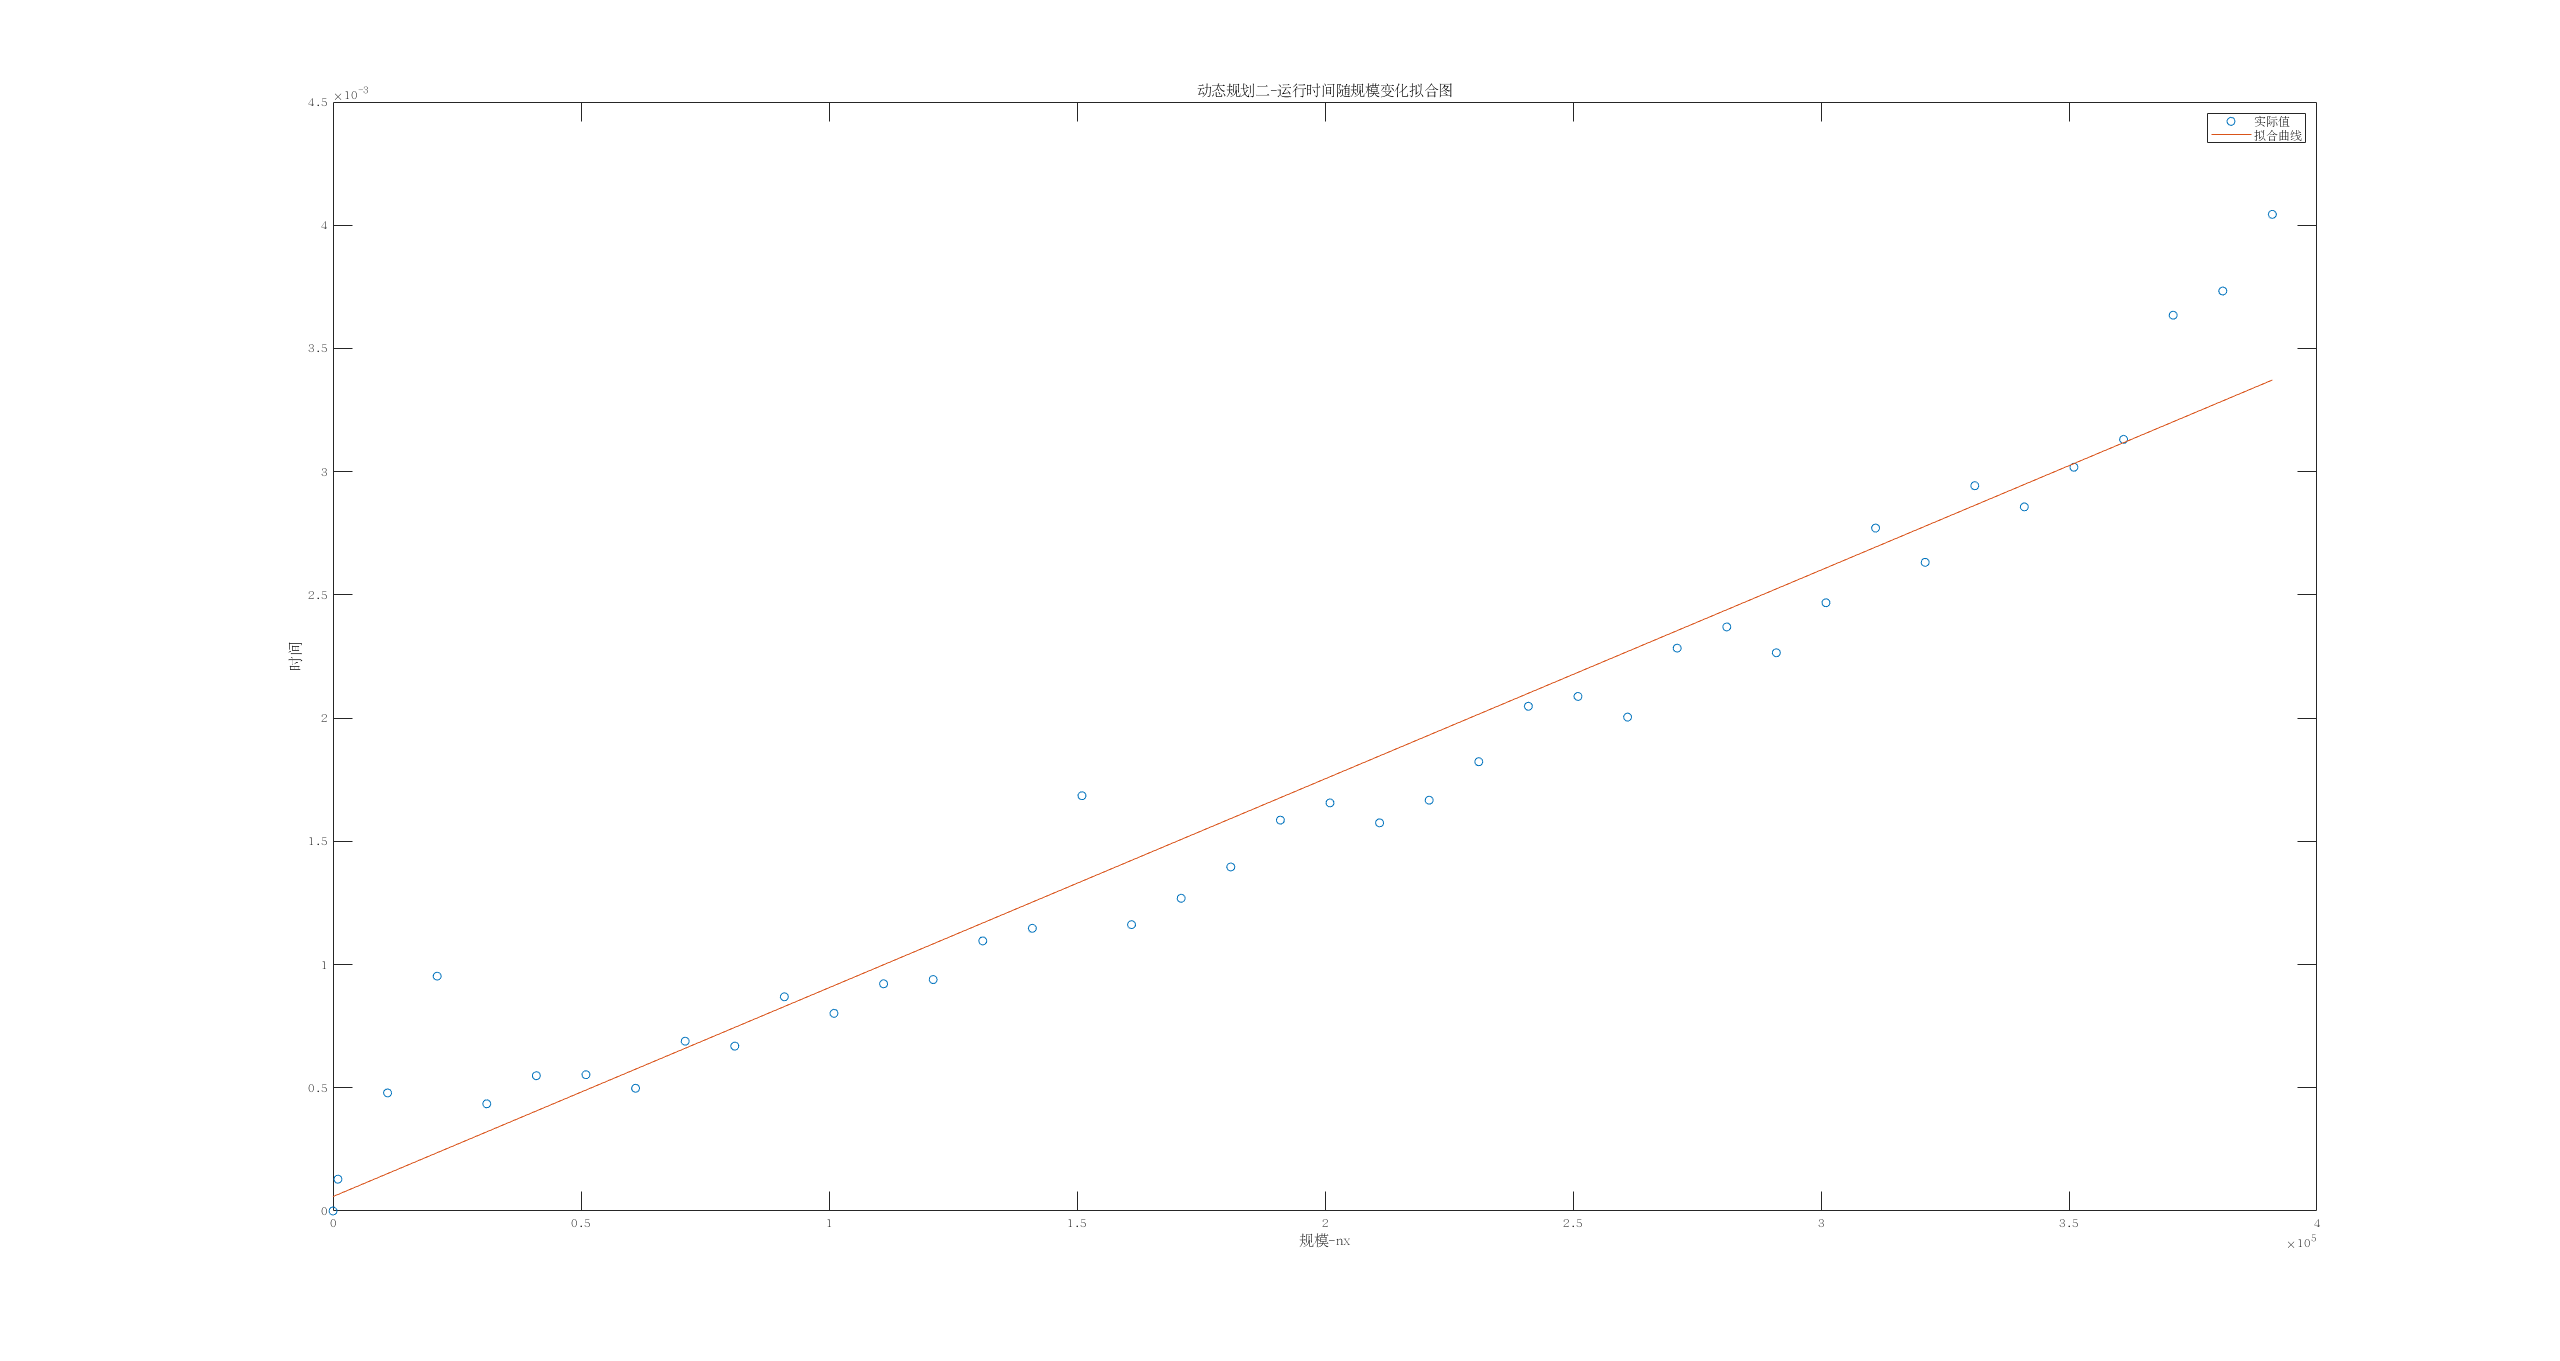
\includegraphics[width=10cm]{3.png}
        \caption{稀疏点拟合}
    \end{minipage}
    \begin{minipage}[t]{1\textwidth}
        \centering
        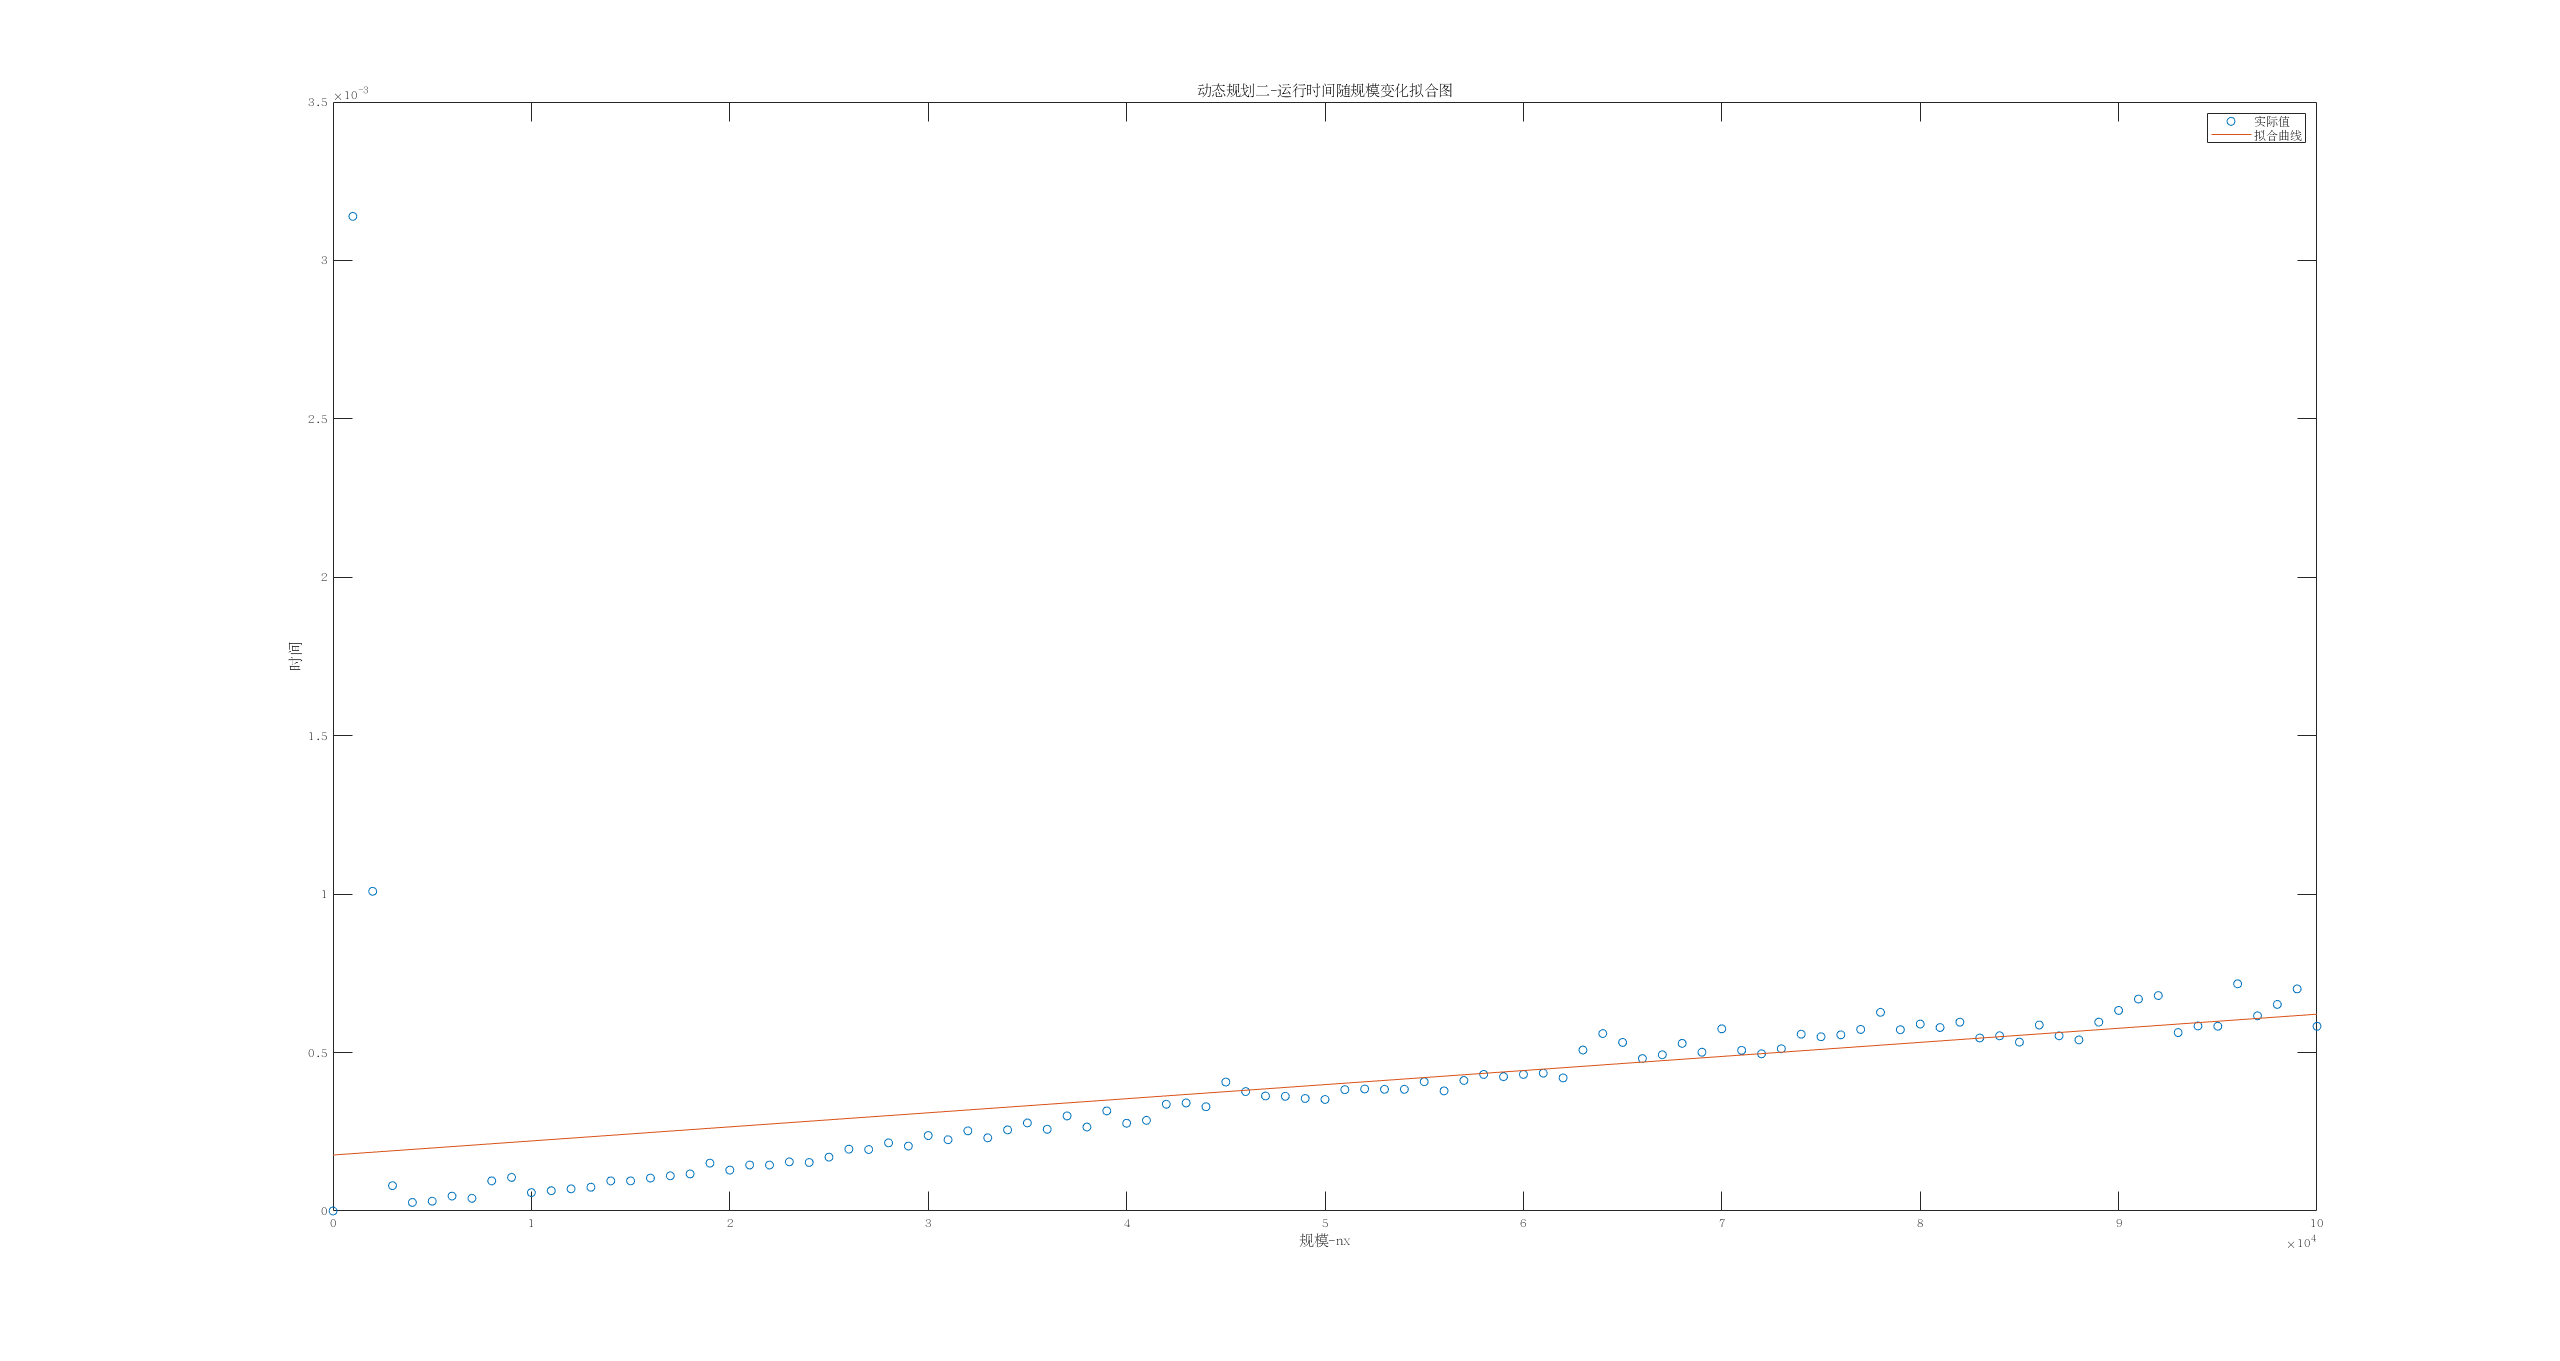
\includegraphics[width=10cm]{4.png}
        \caption{密集点拟合}
    \end{minipage}
\end{figure}


\subsection{实现思路}
步骤:
\begin{itemize}
    \item 预分配内存:使用一个n×(x+1)二维数组temp来存储所有子问题的最优值,以及一个n×(x+1)的0-1二维数组s来存储当前最优方案下是否选择了新增的物品。
    \item 从只有一个物品开始迭代,同时背包容量也从0开始迭代直到x为止。
    \item 在当前物品集合下,当前背包容量下做出是否选择当前物品的决策。并且记录下来
    \item 最后的temp(n,x+1)就是最优值,决策方案根据s给出,具体步骤如下。
\end{itemize}

根据s给出决策方案步骤:
\begin{itemize}
    \item 从s(n,x+1)开始,如果为1,证明选择了第n个物品。如果为0,证明没选。
    \item 如果上一步为1,那么跳到 s(n-1,x+1-v(n)) ,看它为1还是0。如果上一步为0,跳到s(n-1,x+1)进行判断。
    \item 重复上述步骤,直到全部判断完毕,这样就得出了最优方案。
\end{itemize}

代码见knapsack.m附件。


\subsection{测试用例}
思路:寻找已经得到证实的背包问题解,验证自己的算法。

将test.m附件。

\section{两种动态规划的对比}
从实现思路上来说,第一种只对背包的容量进行了“动态规划”,而第二种在对背包容量进行动态规划的同时,也对物品的种类进行了划分。所以针对第一种,我使用了一个一维数组存储最优值,对于第二种,使用了二维的数组。在求解决策方案上,对于第一种,直接将每个子问题的选品方案存在一个二维数组里面,对于第二种,我是从物品的角度来看,如果选择了当前迭代的物品,那么存1,否则存0.

空间复杂度:第一种使用一个一维数组,一个二维数组。第二种动态规划使用两个二维数组。故易知,第二种方案在空间上开销优于第一种。

时间复杂度:两种方案都近似于\(O(nx)\)。但在循环内部,第一种每一次都要查找所有物品,而第二种只用决策是否选择当前物品。故总的来说,第二种动态规划在时间上消耗比第一种少很多。由前面给出了图也看出,第一种的数量级为1,第二种的数量级为\(10^{-4}\)

下面给出图示验证。
\begin{figure}[H] %[htbp]
    \centering
    \begin{minipage}[t]{1\textwidth}
        \centering
        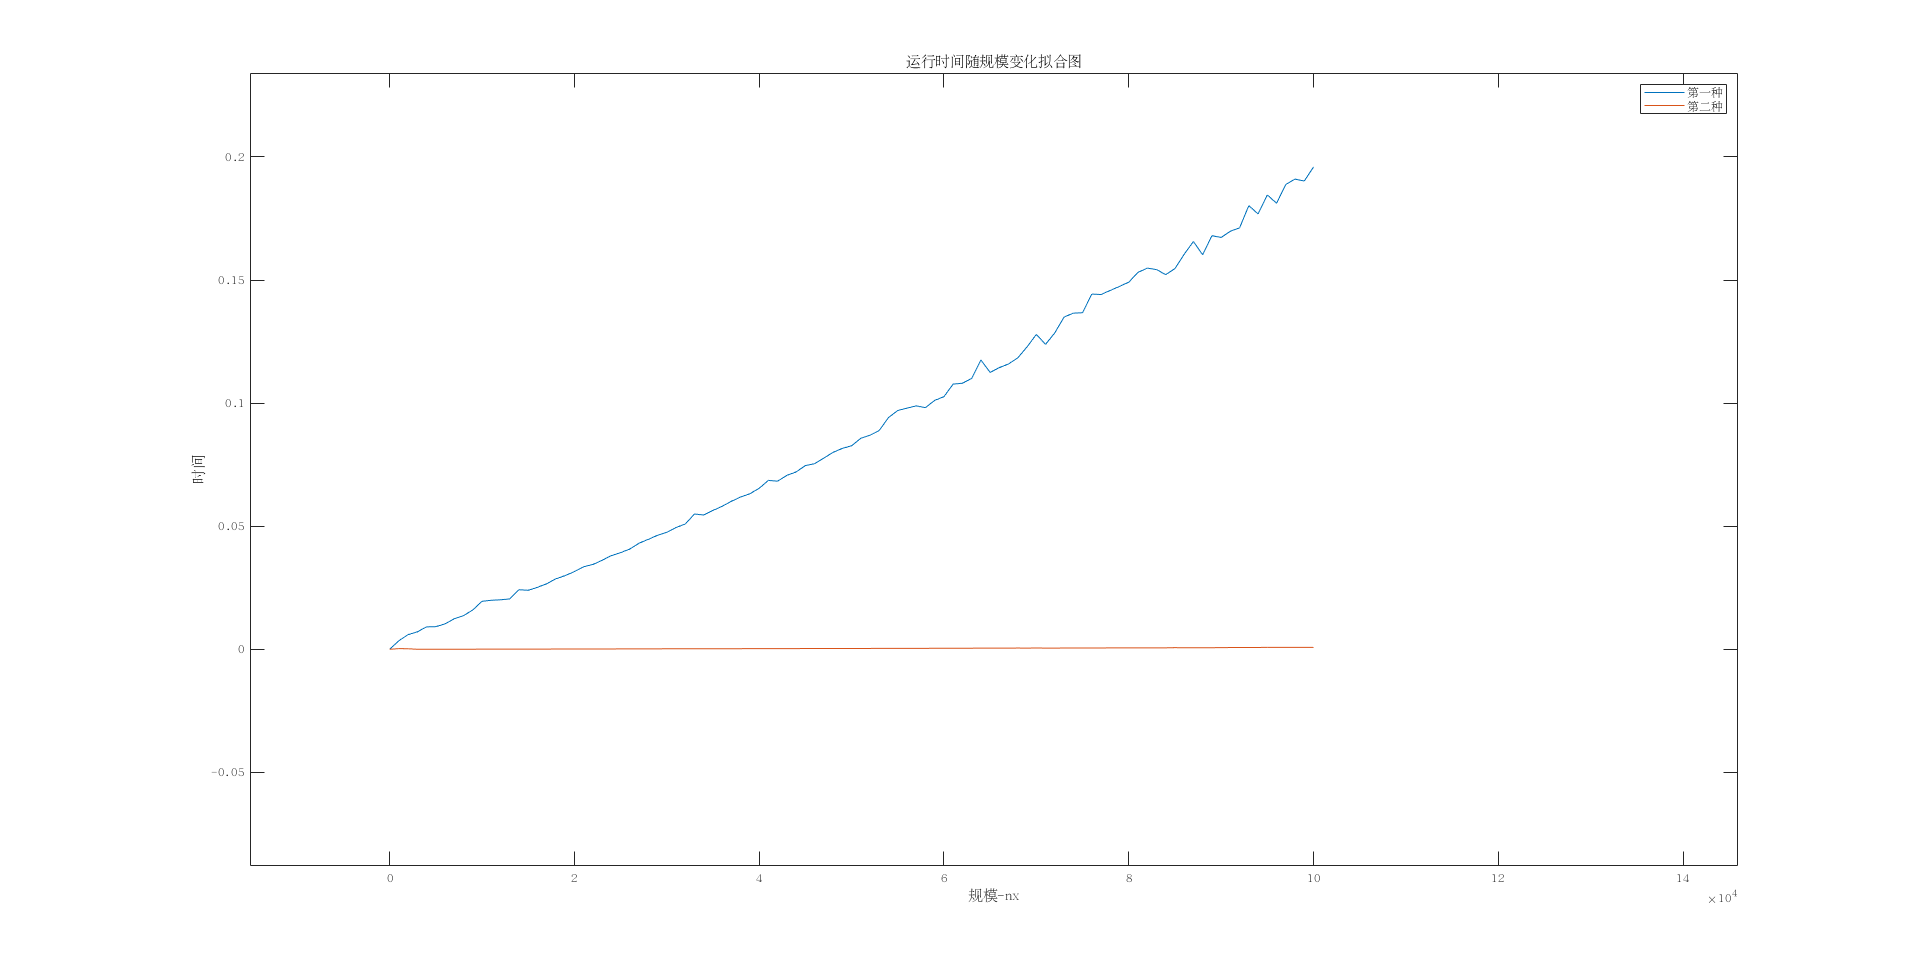
\includegraphics[width=10cm]{5.png}
        \caption{对比}
    \end{minipage}
\end{figure}
\section{启发式:贪婪算法}
\subsection{问题描述}
针对背包问题,一种很自然的想法就是先选择性价比最高的物品,也就是v/w最高的。但是这只是在当前看来是最优的选着,但是对于长远来说,可能存在浪费背包容量的问题,所以这只是一种近似的解法。

\subsection{实现思路}
步骤:
\begin{itemize}
    \item 将物品按找v/w从大到小排序。
    \item 选择当前背包剩余容量能装下的最大性价比的物品。
    \item 重复第二步,直到背包再也装不下任何物品。
\end{itemize}

\subsection{算例分析}
按照问题描述,由于所有的物品都只扫描了一次,所以算法的时间复杂度为\(O(n)\)。

启发的式的贪婪算法虽然得不到问题的最优解,但是其在问题规模较大的时候,能得到比较理想的结果,并且其时间复杂度相比与动态规划大幅降低了。

如下图:
\begin{figure}[H] %[htbp]
    \centering
    \begin{minipage}[t]{1\textwidth}
        \centering
        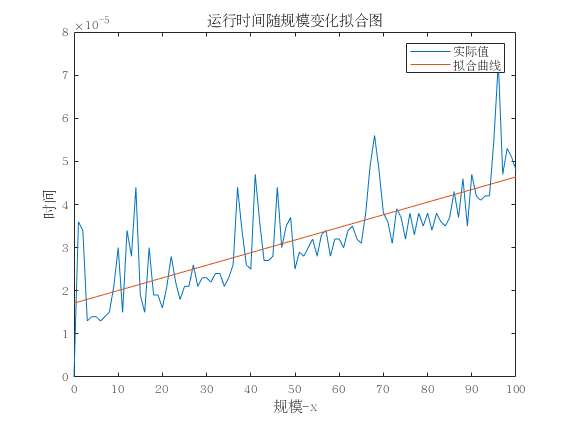
\includegraphics[width=10cm]{10.png}
        \caption{对比}
    \end{minipage}
\end{figure}


\section{总结}
二维的动态规划形式不一定劣于一维的动态规划形式,反而因为它在迭代过程中将大量子问题存储起来,这样在后续计算中能减少很多次的比较,故效率高于一维的动态规划形式。

启发的式的贪婪算法虽然得不到问题的最优解,但是其在问题规模较大的时候,能得到比较理想的结果,并且其时间复杂度相比与动态规划大幅降低了。


\end{document}